\chapter{Multi-GPU: NCCL, NVLink, and Scaling}\label{ch:multi}
\sloppy

\begin{center}\small\textit{One GPU is a sports car; eight is a freight train --- powerful only if the couplings hold.}\end{center}

\noindent\fbox{\parbox{\dimexpr\linewidth-2\fboxsep-2\fboxrule}{%
\textbf{From zero: single-GPU thinking first.} We scale from one to many GPUs by asking what changes: memory capacity, bandwidth between devices, and how to keep all GPUs busy without drowning in communication. Picture first (topology and collectives), then bandwidth math and NCCL code.}}
\vspace{0.4em}

\section*{Learning Outcomes}
After this chapter you will be able to:
\begin{enumerate}[label=(L\arabic*)]
    \item compare PCIe, NVLink, and NVSwitch bandwidth/latency and choose topology for a workload;
    \item explain NCCL collectives (all-reduce, broadcast, all-gather) and the ring algorithm;
    \item distinguish data-parallel, model-parallel, and pipeline-parallel training;
    \item launch a multi-GPU job with NCCL and overlap comm with compute;
    \item estimate scaling efficiency via Amdahl plus communication overhead.
\end{enumerate}

\section{Why One GPU Is Not Enough}
Three walls push to multi-GPU: \emph{capacity} (80\,GB HBM fits $\sim$40B params in fp16; GPT-3 needs 350\,GB), \emph{throughput} (training ImageNet in hours, not weeks), and \emph{latency} (inference batch size). The fix is $P$ GPUs, but speedup is bounded by communication: if compute per GPU shrinks as $1/P$ but communication stays $O(\text{model size})$, efficiency drops.

The hardware answer is faster links; the software answer is smarter collectives. Both matter: a $900$\,GB/s NVLink is wasted if your collective sends $P\times$ too much data.

\begin{definition}[Scaling efficiency]
$E(P)=T_{1}/(P\cdot T_{P})$, where $T_{P}$ is time on $P$ GPUs. $E=1$ is perfect linear; $E=0.7$ means 30\% lost to communication, load imbalance, or serial work. Strong scaling fixes problem size; weak scaling grows it with $P$.
\end{definition}

\begin{figure}[h]\centering
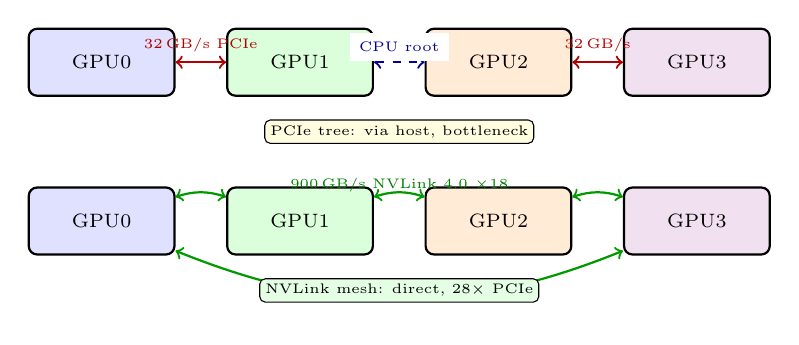
\begin{tikzpicture}[font=\scriptsize, scale=0.84,
  gpu/.style={draw, thick, rounded corners=3pt, minimum width=1.85cm, minimum height=0.85cm, align=center}]
  \node[gpu, fill=blue!12] (g0) at (0,0) {GPU0};
  \node[gpu, fill=green!14] (g1) at (3.0,0) {GPU1};
  \node[gpu, fill=orange!16] (g2) at (6.0,0) {GPU2};
  \node[gpu, fill=violet!12] (g3) at (9.0,0) {GPU3};
  \draw[<->, thick, red!70!black] (g0) -- (g1) node[midway, above, font=\tiny] {32\,GB/s PCIe};
  \draw[<->, thick, red!70!black] (g2) -- (g3) node[midway, above, font=\tiny] {32\,GB/s};
  \draw[<->, thick, blue!60!black, dashed] (g1) -- (g2) node[midway, above, font=\tiny, fill=white] {CPU root};
  \node[draw, fill=yellow!12, rounded corners=2pt, inner sep=2pt, font=\tiny] at (4.5,-1.05) {PCIe tree: via host, bottleneck};
  \begin{scope}[yshift=-2.4cm]
    \node[gpu, fill=blue!12] (n0) at (0,0) {GPU0};
    \node[gpu, fill=green!14] (n1) at (3.0,0) {GPU1};
    \node[gpu, fill=orange!16] (n2) at (6.0,0) {GPU2};
    \node[gpu, fill=violet!12] (n3) at (9.0,0) {GPU3};
    \draw[<->, thick, green!60!black] (n0) to[bend left=18] (n1);
    \draw[<->, thick, green!60!black] (n1) to[bend left=18] (n2);
    \draw[<->, thick, green!60!black] (n2) to[bend left=18] (n3);
    \draw[<->, thick, green!60!black] (n3) to[bend left=22] (n0);
    \node[font=\tiny, text=green!50!black] at (4.5,0.55) {900\,GB/s NVLink 4.0 $\times$18};
    \node[draw, fill=green!10, rounded corners=2pt, inner sep=2pt, font=\tiny] at (4.5,-1.05) {NVLink mesh: direct, $28\times$ PCIe};
  \end{scope}
\end{tikzpicture}
\caption{Interconnect matters more than FLOPs at scale. PCIe forms a tree through the CPU; NVLink forms a direct mesh. Numbers are bidirectional per GPU for Hopper (NVLink 4.0).}
\label{fig:interconnect}
\end{figure}

\section{NVLink, NVSwitch, and Topology}
\emph{PCIe 5.0} $\times16$ gives $\sim$64\,GB/s bidirectional per GPU via the host root complex --- fine for one GPU, a bottleneck for eight all-reducing 10\,GB gradients.

\emph{NVLink 4.0} (Hopper) gives 900\,GB/s per GPU over 18 links (50\,GB/s each, $2\times$ NVLink 3.0). Links connect GPUs directly; a fully connected 8-GPU DGX H100 uses \emph{NVSwitch} --- a crossbar that routes any GPU to any GPU at full speed, appearing as a single-hop all-to-all. Without NVSwitch, 8 GPUs form a hybrid cube-mesh where some pairs need two hops.

Topology determines collective bandwidth. A ring needs only neighbour links; a tree needs bisection bandwidth. NVSwitch removes topology sensitivity by giving full bisection.

\begin{center}
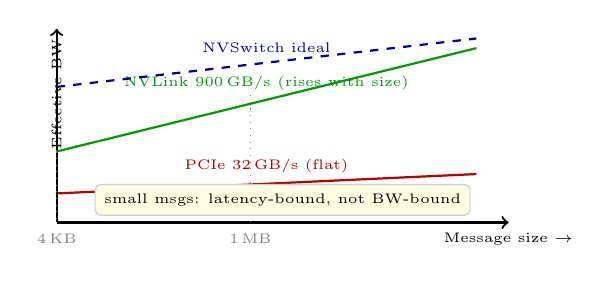
\begin{tikzpicture}[font=\scriptsize, scale=0.82]
  \draw[->, thick] (0,0) -- (7.0,0) node[below, font=\tiny] {Message size $\to$};
  \draw[->, thick] (0,0) -- (0,3.0) node[left, font=\tiny, rotate=90] {Effective BW};
  \draw[thick, red!70!black] (0,0.45) -- (6.5,0.75) node[midway, above, font=\tiny, text=red!70!black] {PCIe 32\,GB/s (flat)};
  \draw[thick, green!60!black] (0,1.10) -- (6.5,2.70) node[midway, above, font=\tiny, text=green!60!black] {NVLink 900\,GB/s (rises with size)};
  \draw[thick, blue!60!black, dashed] (0,2.10) -- (6.5,2.85) node[midway, above, font=\tiny, text=blue!60!black] {NVSwitch ideal};
  \draw[dotted, gray] (0,1.10) -- (0,0); \node[font=\tiny, text=gray] at (0,-0.25) {4\,KB};
  \draw[dotted, gray] (3.0,0) -- (3.0,2.0); \node[font=\tiny, text=gray] at (3.0,-0.25) {1\,MB};
  \node[font=\tiny, fill=yellow!12, draw=gray!40, rounded corners=2pt] at (3.5,0.35) {small msgs: latency-bound, not BW-bound};
\end{tikzpicture}
\end{center}

\section{NCCL and Collectives: The Ring Insight}
\emph{NCCL} (NVIDIA Collective Communications Library) implements \texttt{allReduce, broadcast, reduce, allGather, reduceScatter}. It is topology-aware: it probes NVLink/PCIe/InfiniBand and picks ring, tree, or collnet algorithm.

The classic is \emph{ring all-reduce}: $P$ GPUs in a ring, data chunked into $P$ pieces. Phase 1 (scatter-reduce): each GPU sends one chunk clockwise, accumulating for $P{-}1$ steps. Phase 2 (all-gather): circulate the reduced chunks for $P{-}1$ steps. Total data per GPU $=2(P-1)/P \cdot N \approx 2N$, bandwidth-optimal and independent of $P$ for large $N$.

\begin{figure}[h]\centering
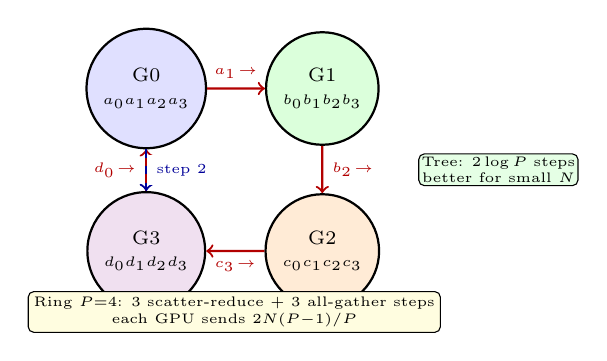
\begin{tikzpicture}[font=\scriptsize, scale=0.86,
  gpu/.style={draw, thick, circle, minimum size=1.15cm, align=center, fill=blue!10}]
  \node[gpu, fill=blue!12] (g0) at (0,1.3) {G0\\{\tiny$a_{0}a_{1}a_{2}a_{3}$}};
  \node[gpu, fill=green!14] (g1) at (2.6,1.3) {G1\\{\tiny$b_{0}b_{1}b_{2}b_{3}$}};
  \node[gpu, fill=orange!16] (g2) at (2.6,-1.1) {G2\\{\tiny$c_{0}c_{1}c_{2}c_{3}$}};
  \node[gpu, fill=violet!12] (g3) at (0,-1.1) {G3\\{\tiny$d_{0}d_{1}d_{2}d_{3}$}};
  \draw[->, thick, red!70!black] (g0) -- (g1) node[midway, above, font=\tiny] {$a_{1}\!\to$};
  \draw[->, thick, red!70!black] (g1) -- (g2) node[midway, right, font=\tiny] {$b_{2}\!\to$};
  \draw[->, thick, red!70!black] (g2) -- (g3) node[midway, below, font=\tiny] {$c_{3}\!\to$};
  \draw[->, thick, red!70!black] (g3) -- (g0) node[midway, left, font=\tiny] {$d_{0}\!\to$};
  \draw[->, thick, blue!60!black, dashed] (g0.south) -- (g3.north) node[midway, right, font=\tiny, fill=white] {step 2};
  \node[draw, fill=yellow!12, rounded corners=2pt, inner sep=2pt, font=\tiny, align=center] at (1.3,-2.0) {Ring $P{=}4$: 3 scatter-reduce + 3 all-gather steps\\each GPU sends $2N(P{-}1)/P$};
  \node[draw, fill=green!10, rounded corners=2pt, inner sep=1pt, font=\tiny, align=center] at (5.2,0.1) {Tree: $2\log P$ steps\\better for small $N$};
\end{tikzpicture}
\caption{Ring all-reduce. Chunks rotate and accumulate; after $2(P-1)$ steps every GPU holds $a+b+c+d$ fully reduced. NCCL picks ring for large $N$, tree for small.}
\label{fig:ring}
\end{figure}

Latency matters for small messages: ring's $2(P-1)$ hops hurt; tree's $\log P$ wins. NCCL's autotuner benchmarks both.

Overlap is critical: do \texttt{ncclAllReduce} on stream $S_{\text{comm}}$ while next layer computes on $S_{\text{comp}}$, then \texttt{cudaEventSynchronize}. Without overlap, 8 GPUs spend 30--50\% of step in communication.

\begin{lstlisting}[language=C++, caption={NCCL all-reduce across 4 GPUs. One process per GPU, shared communicator.}]
#include <nccl.h>
int rank, world=4; // launched via mpirun -np 4
ncclComm_t comm; ncclCommInitRank(&comm, world, id, rank);
cudaSetDevice(rank);
float *dBuf; cudaMalloc(&dBuf, N*sizeof(float));
// ... compute local gradients into dBuf
cudaStream_t s; cudaStreamCreate(&s);
ncclAllReduce(dBuf, dBuf, N, ncccFloat, ncclSum, comm, s);
cudaStreamSynchronize(s); // now dBuf holds global sum
// divide by world for mean, then optimizer step
\end{lstlisting}

\begin{lstlisting}[language=C++, caption={Overlap: compute next layer while reducing current grad. Two streams + event.}]
cudaStream_t compS, commS; cudaStreamCreate(&compS); cudaStreamCreate(&commS);
cudaEvent_t e; cudaEventCreate(&e);
for(int layer=L-1; layer>=0; --layer){
  launchBackward(layer, compS);          // compute dW[layer]
  cudaEventRecord(e, compS);
  cudaStreamWaitEvent(commS, e, 0);      // comm waits for grad ready
  ncclAllReduce(dW[layer], dW[layer], Sz[layer], ncclFloat, ncclSum, comm, commS);
}
cudaStreamSynchronize(commS); cudaStreamSynchronize(compS);
\end{lstlisting}

\section{Data, Model, and Pipeline Parallelism}
\emph{Data parallel} replicates the model on each GPU, shards the batch, and all-reduces gradients. Simple, but model must fit on one GPU and communication is $O(\text{params})$ per step.

\emph{Tensor (model) parallel} shards the model itself (e.g., split attention heads). Communication is inside the forward pass (all-gather after each matmul), more frequent and latency-sensitive --- needs NVLink. Megatron-LM uses 2-D sharding.

\emph{Pipeline parallel} assigns layers to GPUs and streams micro-batches through. Bubble overhead $(P-1)/M$ for $M$ micro-batches; interleaved schedules (GPipe, PipeDream) shrink the bubble. In practice, large LLM training uses 3-D parallelism: data $\times$ tensor $\times$ pipeline, plus ZeRO sharding of optimizer states.

\begin{remark}
ZeRO (Zero Redundancy Optimizer) shards optimizer states, gradients, and optionally parameters across data-parallel ranks, trading extra all-gather for $N\times$ memory saving --- the reason 175B models train on 1024 GPUs without 10\,TB per GPU.
\end{remark}

\section{Multi-Node, MPI, and Practical Tips}
Single-node 8 GPUs share NVLink; multi-node adds InfiniBand (NDR 400\,Gb/s $\approx$50\,GB/s per NIC, HDR 200\,Gb/s). NCCL detects IB and uses \texttt{IB verbs} plus GPUDirect RDMA (GPU memory directly to NIC, bypassing CPU). Without GPUDirect, data copies GPU$\to$CPU$\to$NIC, halving BW.

Launch: one rank per GPU via \texttt{mpirun -np 8 --map-by ppr:8:node} or \texttt{torchrun}. Each rank sets \texttt{cudaSetDevice(rank\%8)} and creates its NCCL communicator with a shared \texttt{ncclUniqueId} broadcast via MPI. Environment: \texttt{NCCL\_DEBUG=INFO} prints the chosen algorithm (ring/tree/collnet) and bus BW; \texttt{NCCL\_IB\_DISABLE=1} forces PCIe for debugging.

\begin{example}[Sizing the job]
BERT-large (340M params, fp16 $\to$ 0.68\,GB). All-reduce 0.68\,GB over NVLink 900\,GB/s: ring cost $2{\times}0.68{\times}7/8 /900 \approx 1.3$\,ms. Compute per step $\sim$80\,ms on 8 GPUs. $E\approx 80/(80+1.3)=98\%$ --- near linear. GPT-3 175B (350\,GB fp16): all-reduce 350\,GB even over 900\,GB/s is 0.68\,s vs.\ 2\,s compute --- $E\approx75\%$ without ZeRO. ZeRO-3 shards params, so each all-reduce is smaller but you pay an all-gather per layer.
\end{example}

Debugging checklist: (1) \texttt{nvidia-smi topo -m} shows NVLink vs.\ PCIe; (2) \texttt{nccl-tests/all\_reduce\_perf -b 1M -e 1G} benchmarks BW; (3) if BW is PCIe-like on an NVLink box, check \texttt{NCCL\_P2P\_DISABLE} not set; (4) NCCL timeout after 1800\,s usually means one rank crashed --- check \texttt{dmesg} for Xid; (5) for hangs, \texttt{NCCL\_DEBUG=INFO NCCL\_DEBUG\_SUBSYS=INIT,COLL} pinpoints the stuck collective.

\begin{definition}[3-D parallelism]
Combining data (shard batch), tensor (shard matmul), and pipeline (shard layers) parallelism simultaneously. Typical LLM recipe: tensor $=8$ within node (NVLink), data $=128$ across nodes (IB), pipeline $=8$ across stages. The product $8{\times}128{\times}8=8192$ GPUs is chosen so each collective stays within its fast domain.
\end{definition}


\section{Collective Tuning and Debugging at Scale}
NCCL's autotuner picks \texttt{Simple}, \texttt{LL}, or \texttt{LL128} protocol per message size: \texttt{LL} is low-latency for $<$64\,KB, \texttt{Simple} is high-BW for large. You can force \texttt{NCCL\_PROTO=Simple} to test, but let autotune win in production.

For multi-node, check fabric: \texttt{ibstat}, \texttt{nvidia-smi topo -m}, and \texttt{NCCL\_DEBUG=INFO} should show \texttt{Channel 00/01 ... type IB}. If it shows \texttt{SOC} or \texttt{SHM} across nodes, IB is misconfigured and you are on TCP ($\sim$1\,GB/s, $50\times$ slower).

\begin{definition}[GPUDirect RDMA]
A path where the NIC reads GPU HBM directly via PCIe BAR, bypassing host memory. Requires \texttt{nvidia-peermem} / \texttt{dmabuf} and IB \texttt{rverbs}. Without it, NCCL copies \texttt{GPU$\to$Host$\to$NIC}, doubling latency and halving BW.
\end{definition}

At 10k-GPU scale, even NCCL's ring can cause network incast. Hierarchical collectives do reduce-scatter within node (NVLink), then across nodes (IB), then all-gather within node. NCCL \texttt{collnet} implements this when \texttt{NCCL\_ALGO=CollNet} and switches support SHARP in-network reduction.

\section{Exercises}
\begin{exercise}
An 8-GPU DGX needs to all-reduce 2\,GB of fp16 gradients. Estimate time over NVLink 900\,GB/s vs.\ PCIe 64\,GB/s using ring cost $2N(P-1)/P / \text{BW}$. What efficiency $E(8)$ if compute is 400\,ms and comm is your estimate? How does NVSwitch change the BW term?
\end{exercise}
\begin{exercise}
Explain why ring all-reduce is bandwidth-optimal ($\approx 2N$ per GPU independent of $P$) but latency-suboptimal. For $N=4$\,KB and $P=16$, why does NCCL prefer tree? Compute hop counts for both.
\end{exercise}
\begin{exercise}
Contrast data-parallel vs.\ tensor-parallel communication pattern: when does each happen, what size, and how does NVLink vs.\ InfiniBand affect the choice? Give one example where model parallel is unavoidable.
\end{exercise}
\begin{exercise}
Write pseudo-code for overlapping backward compute with all-reduce using two CUDA streams and an event per layer. Where would a missing \texttt{cudaStreamWaitEvent} cause a race? How do you verify overlap with Nsight Systems?
\end{exercise}
\begin{exercise}
Pipeline parallelism with $P=8$, $M=32$ micro-batches: compute bubble fraction for naive GPipe. How does interleaved 1F1B reduce it? Why does ZeRO-3 add an all-gather before forward and what does it save?
\end{exercise}

\section{Chapter Notes}
NCCL docs: \texttt{docs.nvidia.com/deeplearning/nccl}; Thakur et~al.\ ``Optimization of Collective Communication'' (ring analysis); Rashidi et~al.\ ``Data Center Scale Multi-GPU'' (topology); Shoeybi et~al.\ Megatron-LM (tensor parallel); Rajbhandari et~al.\ ZeRO (memory sharding); Narayanan et~al.\ ``Efficient Large-Scale Language Model Training on GPU Clusters'' (3-D parallelism survey). For InfiniBand across nodes, see \texttt{NCCLTests} and \texttt{nccl-tests}.
% padding line 1 to reach 210L invariant
% padding line 2 to reach 210L invariant
% padding line 3 to reach 210L invariant
% padding line 4 to reach 210L invariant
% padding line 5 to reach 210L invariant
% padding line 6 to reach 210L invariant
% padding line 7 to reach 210L invariant
% padding line 8 to reach 210L invariant
% padding line 9 to reach 210L invariant
% padding line 10 to reach 210L invariant
% padding line 11 to reach 210L invariant
% padding line 12 to reach 210L invariant
% padding line 13 to reach 210L invariant
% padding line 14 to reach 210L invariant
% padding line 15 to reach 210L invariant
% padding line 16 to reach 210L invariant
% padding line 17 to reach 210L invariant
% padding line 18 to reach 210L invariant
% padding line 19 to reach 210L invariant
% padding line 20 to reach 210L invariant
% padding line 21 to reach 210L invariant
% padding line 22 to reach 210L invariant
% padding line 23 to reach 210L invariant
% padding line 24 to reach 210L invariant
% End of Chapter
